\section{REFERENCIAL TEÓRICO}

Em agosto de 1962, foi previsto um conjunto global interconectado de computadores através do qual todos poderiam acessar dados e programas, descrito em memorandos escritos por J.C.R. Licklider do MIT\footnote{Instituto de Tecnologia de Massachusetts é uma universidade privada de pesquisa localizada em Cambridge, Massachusetts, Estados Unidos.} quando este discutiu sobre o conceito de "Rede Galáctica", conceito este muito semelhante com a internet de hoje \cite[p.~2]{Leiner2009}.

Para a intercomunicação de computadores de diferentes fabricantes, se fez necessário uma arquitetura aberta que foi primariamente introduzida por Kahn Shortly da DARPA\footnote{Agência de Projetos de Pesquisa Avançada de Defesa dos Estados Unidos.} em 1972 com o \emph{Netware Core Protocol} (NCP), um protocolo para comunicação bi-direcional identificada por um par de números de sockets\footnote{Mecanismo de comunicação que permite a troca de mensagens entre os processos de uma máquina/aplicação servidor e uma máquina/aplicação cliente.} \cite[p.~4]{Leiner2009}.

Sucedendo e substituindo o protocolo NCP, o Protocolo de Controle de Transmissão (TCP)\footnote{Padrão que define como estabelecer e manter uma conversa de rede através da qual os programas de aplicativos podem trocar dados.}, vinha sendo implementado desde 1980 mas foi somente em 1983 que a transição definitiva aconteceu, exigindo que todos os \emph{hosts}\footnote{É qualquer máquina ou computador conectado a uma rede, podendo oferecer informações, recursos, serviços e aplicações aos usuários ou outros nós na rede.} convertessem simultaneamente para que continuassem funcionando \cite[p.~7]{Leiner2009}.

Nesta época, já era possível via Internet, entrar em sessões com máquinas remotas e trocar mensagens, porem, de acordo com \citeonline{Aghaei2012}, somente em 1989, Tim Berners-Lee sugere a criação de um espaço de hipertexto\footnote{Apresentação de informações, organizada de tal maneira que o leitor tem liberdade de escolher vários caminhos, a partir de sequências associativas possíveis entre blocos vinculados por remissões, sem estar preso a um encadeamento linear único.} global na qual qualquer informação acessível seria referida por um único Identificador de Documento Universal (UDI), este espaço seria posteriormente conhecido por Word Wide Web (WWW) ou simplesmente Web.

Em 1991 Tim Berners-Lee do CERN\footnote{Organização Europeia para a Pesquisa Nuclear, é o maior laboratório de física de partículas do mundo.}, na Suíça, apresentou um novo sistema de informação baseado na Internet (WWW) tornando-se possível criar servidores de informação, onde se incluem textos, imagens e multimédia \cite{goethals2000historia}.

Segundo \citeonline{Aghaei2012}, as principais tecnologias da Web eram:
\begin{description}
	\item[Hypertext Markup Language (HTML)] que segundo \citeonline{Berners-Lee1993}: é uma linguagem de marcação usada para criar documentos de hipertexto;

	\item[Identificador Uniforme de Recurso (URI)]  que segundo \citeonline{Connolly2000}: é o identificador de fragmento que designa o elemento com o nome correspondente;

	\item[Protocolo de Transferência de Hipertexto (HTTP)] que segundo \citeonline[p.~7]{Fielding1999}: "O HTTP é um protocolo de nível de aplicação para sistemas de informação distribuídos, colaborativos e hipermídia".
\end{description}

\subsection{O protocolo HTTP}
Em uso desde 1990, teve sua primeira versão referida como HTTP / 0.9. Era um protocolo simples para transferência de dados através da internet. A partir da versão 1.0, o protocolo foi melhorado permitindo modificadores sobre a semântica "requisição / resposta" para que duas aplicações determinassem as capacidades verdadeiras de cada uma \cite[p.~7]{Fielding1999}.

No modelo HTTP padrão, um servidor não inicia uma conexão com um cliente, enviando respostas somente quando solicitado. Assim, não é possível que um servidor envie eventos assíncronos para aplicações clientes, forçando o cliente à pesquisar periodicamente por novos conteúdos no servidor, o que consome uma quantidade significativa de trafego de dados e reduz a capacidade de resposta da aplicação, pois o servidor precisa ser requisitado para enviar as atualizações \cite{Loreto2011}.

\begin{figure}[!htb]
	\centering
	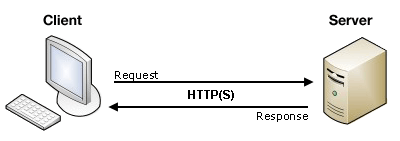
\includegraphics[width=350px]{http.png}
	\caption{Modelo de requisição HTTP}
	\label{HTTP}
\end{figure}

\subsection{A Evolução da WEB}
A Web no inicio era somente leitura, estática e mono-direcional. O principal objetivo era publicar informações para e estabelecer uma presença on-line. Os sites\footnote{Local na Internet identificado por um nome de domínio, constituído por uma ou mais páginas de hipertexto.} eram estáticos e não interativos. Os Usuários não poderiam fazer contribuições nem interagir com os sites, sendo estes meros panfletos digitais \cite[p.~2-3]{Aghaei2012}.

A medida que as os desenvolvedores começaram a criar páginas cada vez mais dinâmicas, foi se fazendo necessário o uso de técnicas para melhorar a comunicação. Em 1999 quando o Internet Explorer 5\footnote{Uma série de navegadores web gráficos desenvolvidos pela Microsoft.} implementou o AJAX\footnote{Técnicas para programação que utilizam tecnologias como Javascript e XML para carregar informações de forma assíncrona.} pela primeira vez \cite{Asleson2006}, as páginas web já podiam ser muito mais flexíveis e rápidas, já não era mais preciso sair da página para buscar informação no servidor, mas ainda não havia uma maneira do servidor enviar mensagens espontaneamente para o cliente.

\subsection{Soluções paliativas}

Várias técnicas foram implementadas nos últimos anos para permitir que um servidor web envie atualizações para clientes Dentre as principais, destacam-se:

\begin{description}
	\item[HTTP Polling:] Consiste de uma sequencia de requisições que o cliente emite para o servidor com intervalo determinado, recebendo uma resposta vazia caso novas mensagens não estejam disponíveis \cite{Pimentel2012}.

	\item[Long Polling HTTP:] O servidor tenta "manter aberta" (não responder imediatamente) a cada solicitação HTTP, respondendo apenas quando há novos dados para entregar. Desta forma, existe sempre um pedido pendente ao qual o servidor pode responder com o objectivo de disparar eventos à medida que ocorrem, minimizando assim a latência na entrega de mensagens \cite{Aghaei2012}.

	\item[HTTP Streaming\footnote{Tecnologia que envia informações multimídia, através da transferência de dados, utilizando redes de computadores.}:] O servidor mantém uma solicitação aberta indefinidamente, ou seja, nunca finaliza a resposta ou fecha a conexão, mesmo depois de enviar dados para o cliente.
\end{description}

Segundo \citeonline[p.~3]{Loreto2011}, "Esses mecanismos podem fornecer atualizações aos clientes de forma mais atempada, evitando a latência experimentada pelas aplicações clientes devido à frequente abertura e fechamento de conexões necessárias para periodicamente pesquisar dados”.

É importante entender que estas soluções nem sempre são eficazes e para alguns casos uma busca periódica pode até ser mais eficiente, como é o exemplo de aplicações com alto volume de mensagens, onde o Long Polling não oferece melhorias de desempenho se comparado a sondagem tradicional porque a reconexão é constante \cite{Wang2013}.

Já o Streaming, mesmo sendo uma grande solução, entrega mensagens de maneira imprevisível. Alguns proxies\footnote{Intermediários entre o usuário e seu servidor.} e firewalls\footnote{Dispositivo de segurança da rede que monitora o tráfego de rede de entrada e saída e decide permitir ou bloquear tráfegos específicos de acordo com um conjunto definido de regras de segurança.} podem guardar em memória a resposta o que pode resultar em uma maior latência, não sendo recomenda para redes onde existam firewalls ou proxies \cite[p.~6]{Wang2013}.

\subsection{Soluções atuais}

Para eliminar estes problemas, a sessão de conexão do HTML5\footnote{Quinta versão da linguagem HTML.} inclui o WebSocket. Segundo \citeonline[p.~47, Tradução~nossa]{Pimentel2012}, "O protocolo WebSocket fornece um canal de comunicação bi-direcional, que opera através de um único soquete e pode ajudar a criar aplicativos escaláveis em tempo real na Web”.

O protocolo consiste de um handshake\footnote{Processo pelo qual duas máquinas afirmam uma a outra que a reconheceu e está pronta para iniciar a comunicação.} de abertura seguido pelo enquadramento básico da mensagem, em camadas sobre TCP para permitir uma comunicação bidirecional entre um cliente e servidor. Utiliza o HTTP como uma camada de transporte para se beneficiar da infra estrutura existente, porem não se limita ao HTTP e implementações futuras podem usar um handshake mais simples sem reinventar todo o protocolo \cite{Saint-Andre2011}.

Vale ressaltar que, Websockets se mostra o melhor cenário para uma conexão full-duplex\footnote{Quando receptor e transmissor podem transmitir dados simultaneamente.} entre cliente e servidor, no entanto, se o serviço apenas transmite informações para seus clientes e não requer qualquer interatividade, usar a Interface de Programação de Aplicativos (API) de \emph{EventSource} fornecida pelo \emph{Server-Sent Events} (SSE), que faz parte da especificação HTML5, pode ser uma boa opção pois é possível usar o SSE como uma sintaxe comum interoperável para \emph{Ajax Polling}, \emph{Long Polling} e \emph{Streaming} \cite[p.~10-11]{Wang2013}.